\documentclass[11pt]{article}
\usepackage{graphicx}    % needed for including graphics e.g. EPS, PS
\topmargin -1.5cm        % read Lamport p.163
\oddsidemargin -0.04cm   % read Lamport p.163
\evensidemargin -0.04cm  % same as oddsidemargin but for left-hand pages
\textwidth 16.59cm
\textheight 21.94cm 
%\pagestyle{empty}       % Uncomment if don't want page numbers
\parskip 7.2pt           % sets spacing between paragraphs
%\renewcommand{\baselinestretch}{1.5} % Uncomment for 1.5 spacing between lines
\usepackage{amsmath}
\usepackage{amsfonts}
\usepackage{amsthm}
\usepackage{verbatim}
\usepackage{subfigure}
\usepackage{cite}
\parindent 0pt		 % sets leading space for paragraphs
\author{Fermi Ma and Erik Waingarten}
\title{A Linear Programming Approach to Dynamic Optimality}

\newtheorem{theorem}{Theorem}
\newtheorem{lemma}[theorem]{Lemma}
\newtheorem{observation}{Observation}

\begin{document}         
\maketitle

\section{Introduction}

We consider the the points in the plane problem. The problem is defined as follows:

\vbox{
\noindent
\begin{quote}
Given a set $P$ of $n$ points $(x_i,y_i)$ in the $xy$ plane, no two on a common row or column, find the minimal point set $Q \supseteq P$ such that for any two points in $Q$ not on a common row or column, the rectangle they span contains another point in $Q$.
\end{quote}
}

The motivation for this problem comes from the dynamic optimality conjecture, first posed by Sleator and Tarjan \cite{SplayTrees}. The conjecture says that given any binary search tree accessing a set of points $A$ with a cost $C(A)$, the splay tree will perform the same accesses with cost $O(n + C(A))$. The binary search tree can only access elements from the root, traveling down through its children, and it can make a tree rotation at any point is the accesses. The dynamic optimality conjecture says that the splay tree is ``as good'' as any other binary search tree. 

Ever since the conjecture, there has been a search for either a proof to show that splay trees are indeed optimal, or another binary search tree that is optimal. Demaine et Al. showed in \cite{geometryBST} that finding an optimal binary search tree in the offline case (all accesses are given before hand) is equivalent to determining an $O(1)$-approximation for the points on the plane problem.

Point sets $Q$ satisfying the condition that any two points in $Q$ spanning a rectangle contain another point in $Q$ are referred to as \emph{arborally satisfied} point sets.

It is natural to restrict attention to the grid of intersection points ``induced" by the set of points $P$: extend horizontal and vertical lines through each point in $P$ and consider only the $O(n^2)$ intersections of these lines. It is easy to show that in any arborally satisfied point set $P$, points that are not grid intersections can be moved to positions that are. An example of such a grid is given Figure~\ref{fig:instance}.

\begin{figure}
\centering
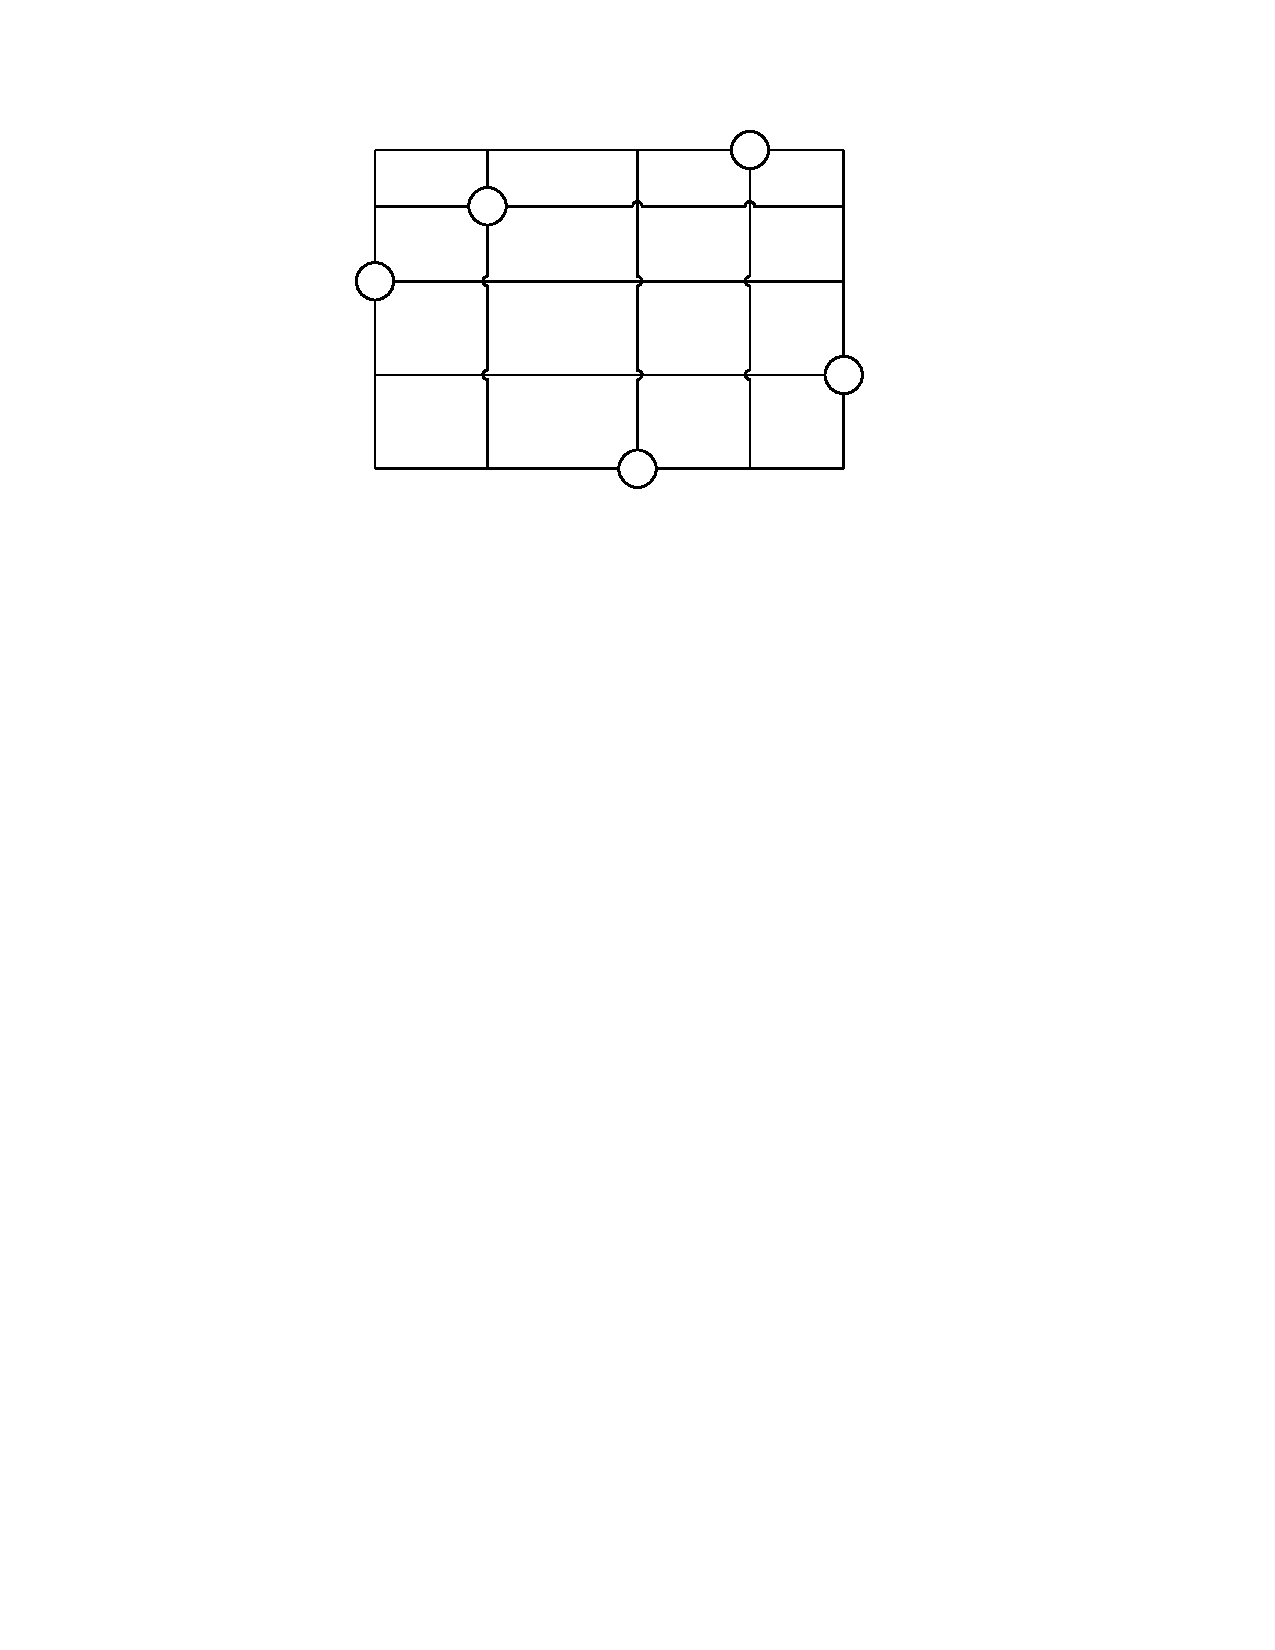
\includegraphics[width=0.3\linewidth]{instance.pdf}
\caption{Instance of points in the plane}
\label{fig:instance}
\end{figure}

We can directly correspond an integer linear program (ILP) to the problem by assigning an indicator variable to each grid point, where the variable is set to 1 if the point is included and is 0 otherwise. This immediately gives us $n$ constraints, one for each variable corresponding to a point in $P$ (setting them all equal to 1). This gives the obvious objective of minimizing the sum of all the variables, and leaves the task of writing down the arboral satisfaction property in terms of other linear constraints. While other linear programming approaches may exist, this setup feels the most natural and so we restrict our attention to it.

We found that it was possible to write down an exact ILP with $O(n^2)$ constraints of size $O(n^2)$, and another ILP with $O(n^2)$ constraints of size $O(n)$ with the same optimal solutions to the original problem. We attempted to use the second ILP formulation to generate an approximation algorithm for the problem by considering the relaxed linear program, but methods such as viewing the problem as a max flow problem and taking the dual proved unsuccessful. Our experiments indicated that the ILP had an integrality gap strictly greater than 1, and we were later able to demonstrate an unbounded integrality gap for the specific ILP we had written down. This indicates that common approximation algorithm for that specific ILP will not work, and we conjecture that an unbounded integrality gap exists for any ILP formulation of the problem. We were not able to prove the conjecture, but we provide some useful observations.

\section{Bounds on the Problem}

Observe that $|Q| = \Omega(n)$ since $P \subset Q$. Furthermore, $|Q| = O(n^2)$ is trivially true since every grid intersection point can be included (see Figure~\ref{fig:instance}). However, there exists a stronger bound (communicated to us verablly by Erik Demaine):

\begin{theorem} $|Q| = O(n\log(n))$
\end{theorem}
\begin{proof}
Let $m$ be the median in the $x$ axis of $P$, this divides $P$ into two sets of size $O(\frac{n}{2})$. Now for each $(x,y) \in P$, let $(m, y) \in Q$. Then recursively solve both subsets of size $O(\frac{n}{2})$. Note that for every two points, they will be divided by the recursion at some point. This means that there is a point in the rectangle. This gives the recursion $|Q| = T(n) = 2T(\frac{n}{2}) + O(n)$, therefore, $|Q| = O(n \log n)$. 
\end{proof}

The same bound arises from viewing each arborally satisfied set as an access sequence of a binary search tree algorithm. \cite{geometryBST}

\section{A First Attempt}

We set up the indicator variables as explained in the introduction, labeling them as $b_{jk}$, where $j$ and $k$ are labels on the grid intersection points (labelled so that $b_{00}$ is the lower left grid point, $b_{01}$ is the point directly above, and $b_{10}$ is the point directly to the right).

Consider the following set of constraints:

\begin{align}
2b_{ij} + 2b_{nm} - \left(\sum_{i \leq k \leq n}\sum_{j\leq l \leq m} b_{kl}\right) &\leq 1  \hspace{.3in} \forall i<n, j<m \\
2b_{im} + 2b_{nj} - \left(\sum_{i \leq k \leq n}\sum_{j\leq l \leq m} b_{kl}\right)  &\leq 1  \hspace{.3in} \forall i<n, m<j
\end{align}

We claim that these constraints exactly capture arboral satisfaction. Constraints of type (1) correspond to all possible ``positive" rectangles, and constraints of type (2) correspond to all possible ``negative" rectangles (explained in Figure 2).

To see the equivalence, first consider constraints of type (1). If points in the grid corresponding to $b_{ij}$ and $b_{nm}$ are present, the rectangle they span must be satisfied by some point corresponding to $b_{kl}$ such that   $i\leq k \leq n$ and $j \leq l \leq m$ (although it cannot equal to $b_{ij}$ or $b_{nm}$). The constraint ensures precisely this: if $b_{ij} = b_{nm} = 1$, at least one other $b_{kl}$ in the parenthesized term must be set to 1, or else the entire left hand side will be a quantity greater than 1. The constraints of type (2) work the same way.

\begin{figure}
\centering
\subfigure[Positive rectangle]{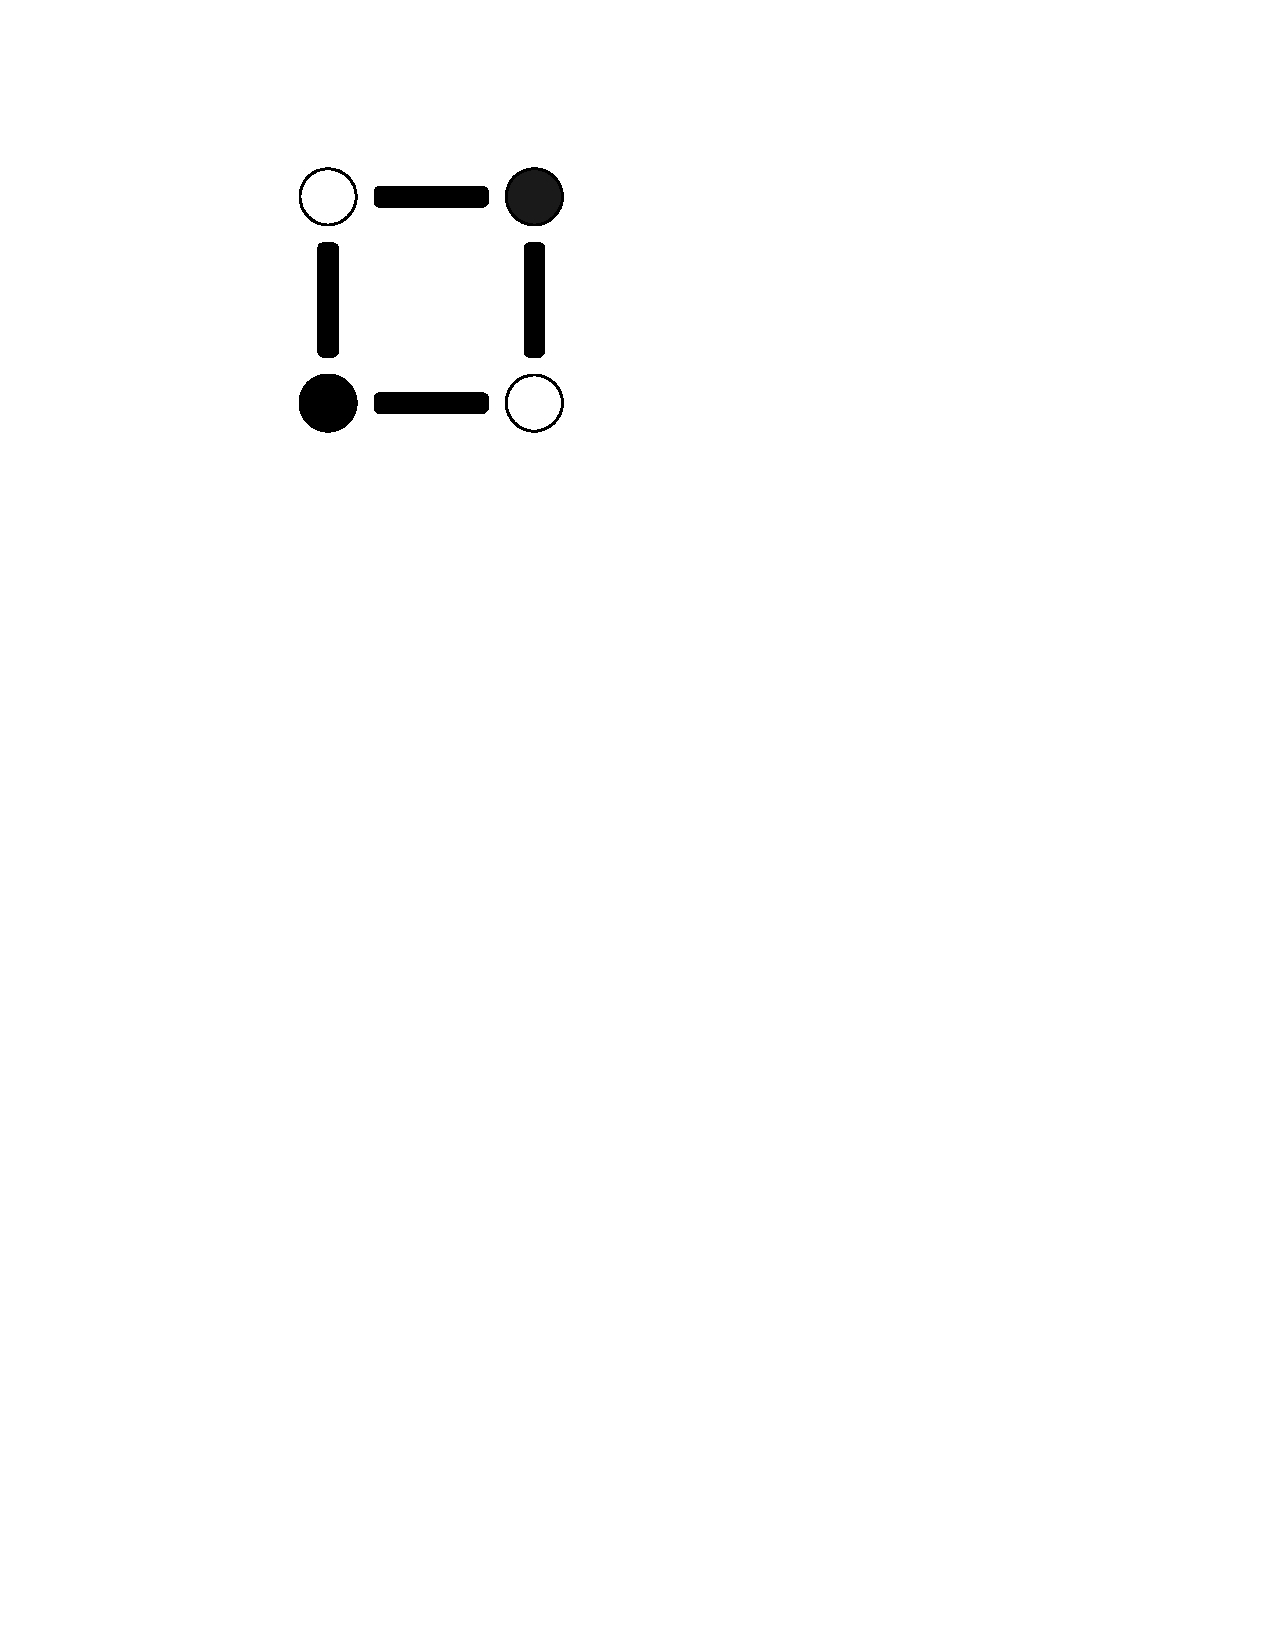
\includegraphics[width=.2\linewidth]{negative.pdf}\label{fig:negative}}
\subfigure[Negative rectangle]{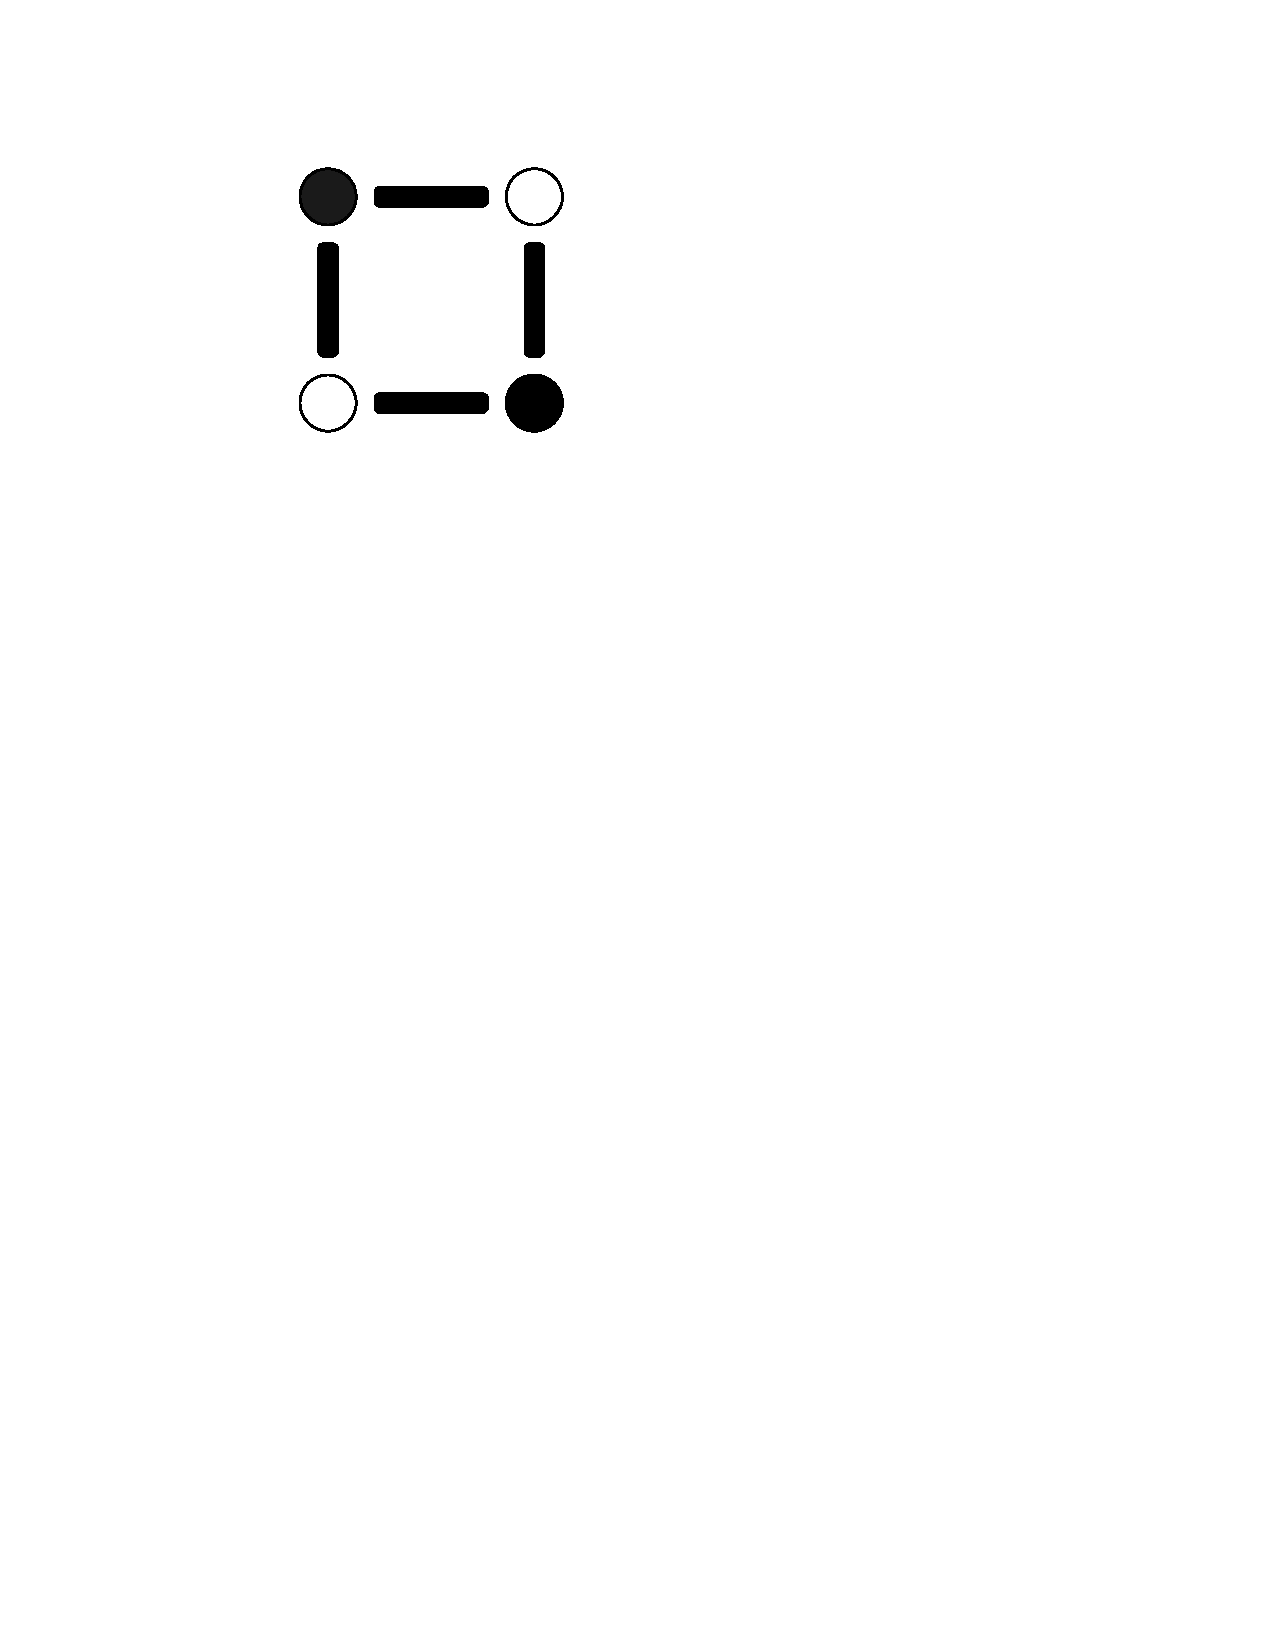
\includegraphics[width=0.2\linewidth]{positive.pdf}\label{fig:positive}}
\caption{Positive and negative rectangles: black corresponds to points that are included, and white corresponds to the points not included}
\label{fig:rectangles}
\end{figure}

\begin{comment}
An easy way to think of the constraints is that we are taking the sum of the points that create a rectangle minus every point inside that rectangle which is not the set points, and that this must be less than 1. This says that if both points of the corners are set to 1, then the sum will be 2, which means that there must be at least one point inside the rectangle set to 1. Thus the rectangle is satisfied. 
\end{comment}
If either of the corner vertices are not present, the rectangle corresponding to the constraint should be inactive, as there does not have to be a point satisfying it. Note that the constraint captures this behavior, since in this case the positive terms will be at most 1, satisfying the inequality no matter what the term in parenthesis is.

If we have such a constraint for every possible rectangle, we will have an arborally satisfied set. Note that this integer linear program will solve for the exact optimal solution.

It turns out that we can simplify the constraints to be linear in size, as we show in Section 4. This seems to be more promising since doing so will decrease the integrality gap. The linear-sized constraints will give an ILP that is exactly equivalent to the ILP given above, but the non-integral solutions to the linear-sized constraint system will turn out to be feasiable solutions to the quadratic-sized constraint system. This will mean that the convex set of solutions for the quadratic-sized constraints will be strictly larger than for the linear-sized constraints, implying a larger integrality gap. 

\section{A Second Attempt: Reducing Constraint Size}
\label{A Second Attempt: Reducing Constraint Size}

By definition, we know that arborally satisfied point sets have all rectangles satisfied by some point on the interior (including edges). It turns out that a short inductive argument shows that all rectangles are in fact satisfied by some point on their edges ~\cite{geometryBST}. This allows us to reduce the size of the constraints from $O(n^2)$ to $O(n)$.

We thus claim that the following set of constraints captures arboral satisfaction: 

\begin{align}
b_{ij} + b_{nm} - \left(\sum_{l=i+1}^{n-1} (b_{lj}+b_{lm}) + \sum_{l=j+1}^{m-1} (b_{il} + b_{nl}) + b_{im} + b_{nj} \right) &\leq& 1 & \hspace{.3in} \forall i<n, j<m \\
b_{im} + b_{nj} - \left(\sum_{l=i+1}^{n-1} (b_{lj}+b_{lm}) + \sum_{l=j+1}^{m-1} (b_{il} + b_{nl}) + b_{ij} + b_{nm} \right) &\leq& 1 & \hspace{.3in} \forall i<n, j<m
\end{align}

Constraints of type (3) correspond to all possible ``positive" rectangles, and constraints of type (4) correspond to all possible ``negative" rectangles. This captures arboral satisfaction for the same reason that the constraints of types (1) and (2) do. The only difference is that we no longer include points that are strictly inside rectangles.

\section{Possible Approaches}

\subsection{Experiments}

We ran experiments to see how the integer linear program compared to the linear program. In particular, we wanted to see whether they were the same, or if there was an the integrality gap greater than 1. We wrote a program in Python that would generate instances of the points in the plane problem and tried to solve it with the second linear program. We used a Python library PuLP which in turn used GLPK (GNU Linear Programming Kit). We were able to run experiments that showed that there are cases for which the second linear program has an integrality gap strictly greater than 1. In all cases, the integrality gap was between 1 and 1.6.

\subsection{Max Flow}

We tried to solve reformulate the ILP as an equivalent flow problem, hoping that this would give a direct solution to the points in the plane problem. We were unsuccessful at coming up with such a formulation, and we believe that no simple max flow formulations of this exact LP exist. A natural way of rewriting this problem as a flow problem would probably result in a flow problem with integral capacities and costs, given that all coefficients in the constraints in the linear program are integers. However, the Integral Flow Theorem would then guarantee that the optimal solution to this LP would be integral. This cannot be the case, since our experimental evidence shows there is an integrality gap strictly greater than 1.

\subsection{The Dual}

The next thing we tried was taking the dual to see if we could derive some alternative combinatorial interpretation for the problem.

Representing the linear program as a matrix, the primal linear program has the objective:
\[ \min \hspace{.1in} [ \begin{array}{cccc} 1 & 1 & \dots & 1 \end{array} ] \left[\begin{array}{c} b_{11} \\ b_{12} \\ \vdots \\ b_{nn} \end{array} \right]\]
with constraints:
\[ \left[ \begin{array}{c} \vdots \\ \text{ $P$ = positive rectangles } \\ \vdots \\ \text{ $N$ = negative rectangles } \\ \vdots \\ \text{ $I_n'$ = equality constraints } \end{array} \right] 
\left[\begin{array}{c} b_{11} \\ b_{12} \\ \vdots \\ b_{nn} \end{array} \right] 
\begin{array}{c} \\ \leq \\ \\ \\ \leq \\ \\ \\ = \end{array} 
\left[\begin{array}{c} 1 \\\\ 1 \\\\ \vdots \\\\ 1 \end{array} \right] \]

where $P$ and $N$ are $\dbinom{n}{2}^2 \times n^2$ matrices, where these values count exactly the number of positive and negative rectangles. $I_n'$ is the some permutation of identity matrix with extra zero columns, and corresponds to the constraints that set variables in the given set of points equal to 1. Furthermore, we require that all variables be positive. 

We compute the dual to be:
\[ \max y^T \left[ \begin{array}{c} 1 \\ 1 \\ \vdots \\ 1 \end{array} \right] \]
such that
\[ \left[ \begin{array}{ccc} \vdots & \vdots & \vdots \\
					  P^T & N^T & I_n \\
					\vdots & \vdots & \vdots \end{array} \right] y
\leq  \left[ \begin{array}{c} 1 \\ 1 \\ \vdots \\ 1 \end{array} \right] \]
Where the first $n$ variables in $y$ can take on any value, and the rest must all be negative. 

This dual gives a somewhat fuzzy combinatorial interpretation:

We have a variable for each rectangle, denoted $r_{ij, lk}$ (corresponding to the rectangle spanned by $b_{ij}$ and $b_{lk}$). Then for each point grid point present corresponding to variable $b_{xy}$, we have the following constraint:
\[ b_{xy} + \sum_{\begin{array}{c}\text{rectangles with}\\\text{$b_{xy}$ on the corner}\end{array}} r_{ij, lk} - \sum_{\begin{array}{c}\text{rectangles with}\\\text{$b_{xy}$ on side}\end{array}} r_{ij,lk} \leq 1 \]
If the grid point is not present, we get the same constraint but without the $b_{xy}$ term. We want to maximize
\[ \sum b_{xy} + \sum r_{ij,lk} \]
where $r_{ij,lk} \leq 0$, and the $b_{xy}$'s are unconstrained. We were unable to find a less convoluted interpretation of the dual than this, so we abandoned the approach.

\section{An Unbounded Integrality Gap}

We were finally able to show that the linear programming relaxation of our ILP (given by constraints (3) and (4)) would not yield an $O(1)$-approximation.

There are known instances of the problem that require $O(n\log n)$ additional points. In any of these instances, we can satisfy the ILP by setting all variables corresponding to neighboring points of points in $P$ to $0.5$ (Refer to Figure 3b for the setup: white circles are variables set to 1, red circles are variables set to 0.5, and empty spots are set to 0).

To see that this solution is feasible, we just check cases. Note that every constraint corresponding to rectangles spanned by points in $P$ will be satisfied, since they contain at least 2 points of value $0.5$. All constraints corresponding to rectangles where one corner is set to $1$ and the opposite corner is set to $0.5$ will satisfied, as at least one other variable of value $0.5$ (adjacent to the corner set to 1) will be subtracted away. Finally each constraint corresponding to a rectangle with opposite corners set to $0.5$ will automatically be satisfied. This feasible solution simply adds 2 to the sum of all the variables for each point in $P$, and is therefore $O(n)$. This implies an integrality gap is $O(\log n)$. 

Figure 3a compares the linear ``solution" of Figure 3b with the optimal solution for a specific instance of the problem. 

\begin{comment}
demonstrates the lower bound of the integrality gap. Figure~\ref{fig:optimum} shows the optimum of the integer linear program, where the white circles are the instance of the problem and the green circles are the variables that are set to 1. It is clear from the picture that all constraints are satisfied and that this is the minimum number of points needed. Figure~\ref{fig:lpsolution} gives a $O(n)$ feasible solution to the linear program where the white circles indicate the instance of the problem and the red circles are the points that are assigned to $0.5$. 
\end{comment}

\begin{figure}
\centering
\subfigure[Optimal solution to integer linear program]{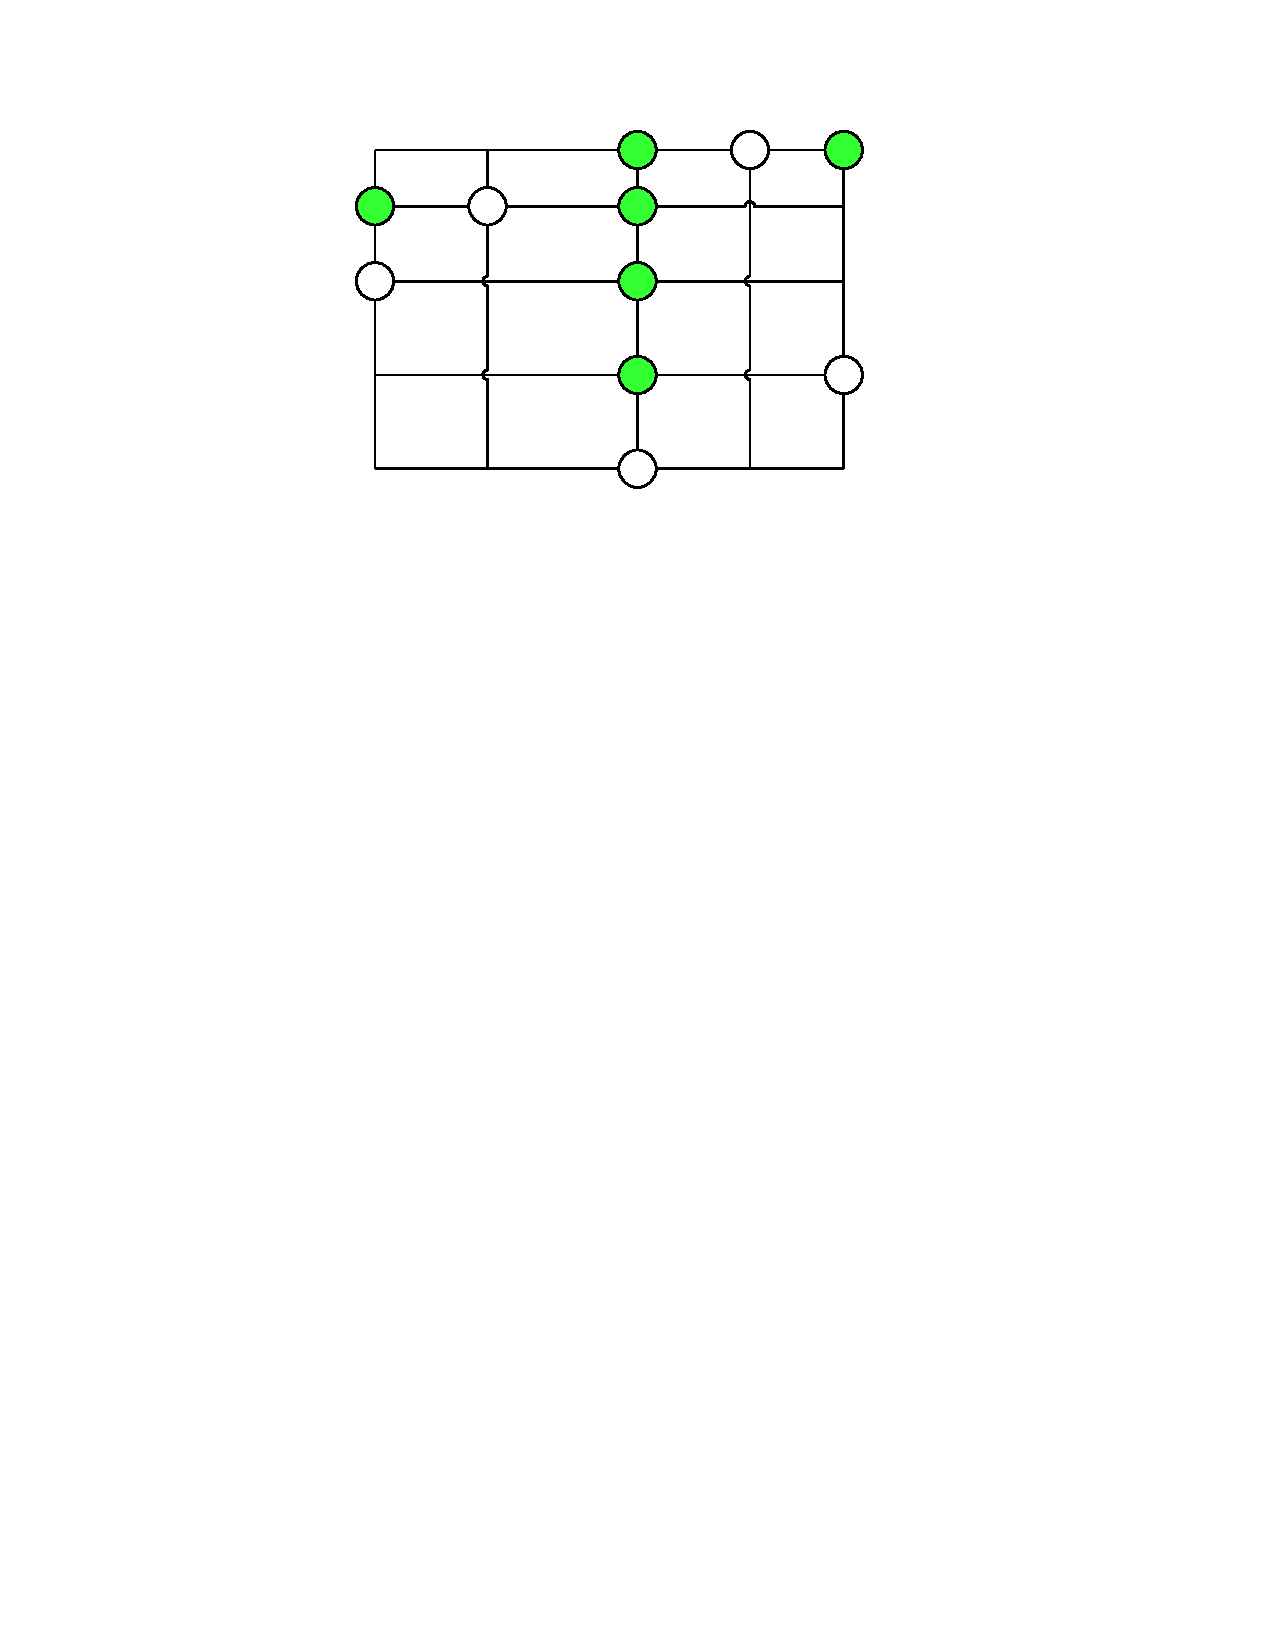
\includegraphics[width=0.4\linewidth]{optimum.pdf}\label{fig:optimum}}
\subfigure[Feasible solution to linear program.]{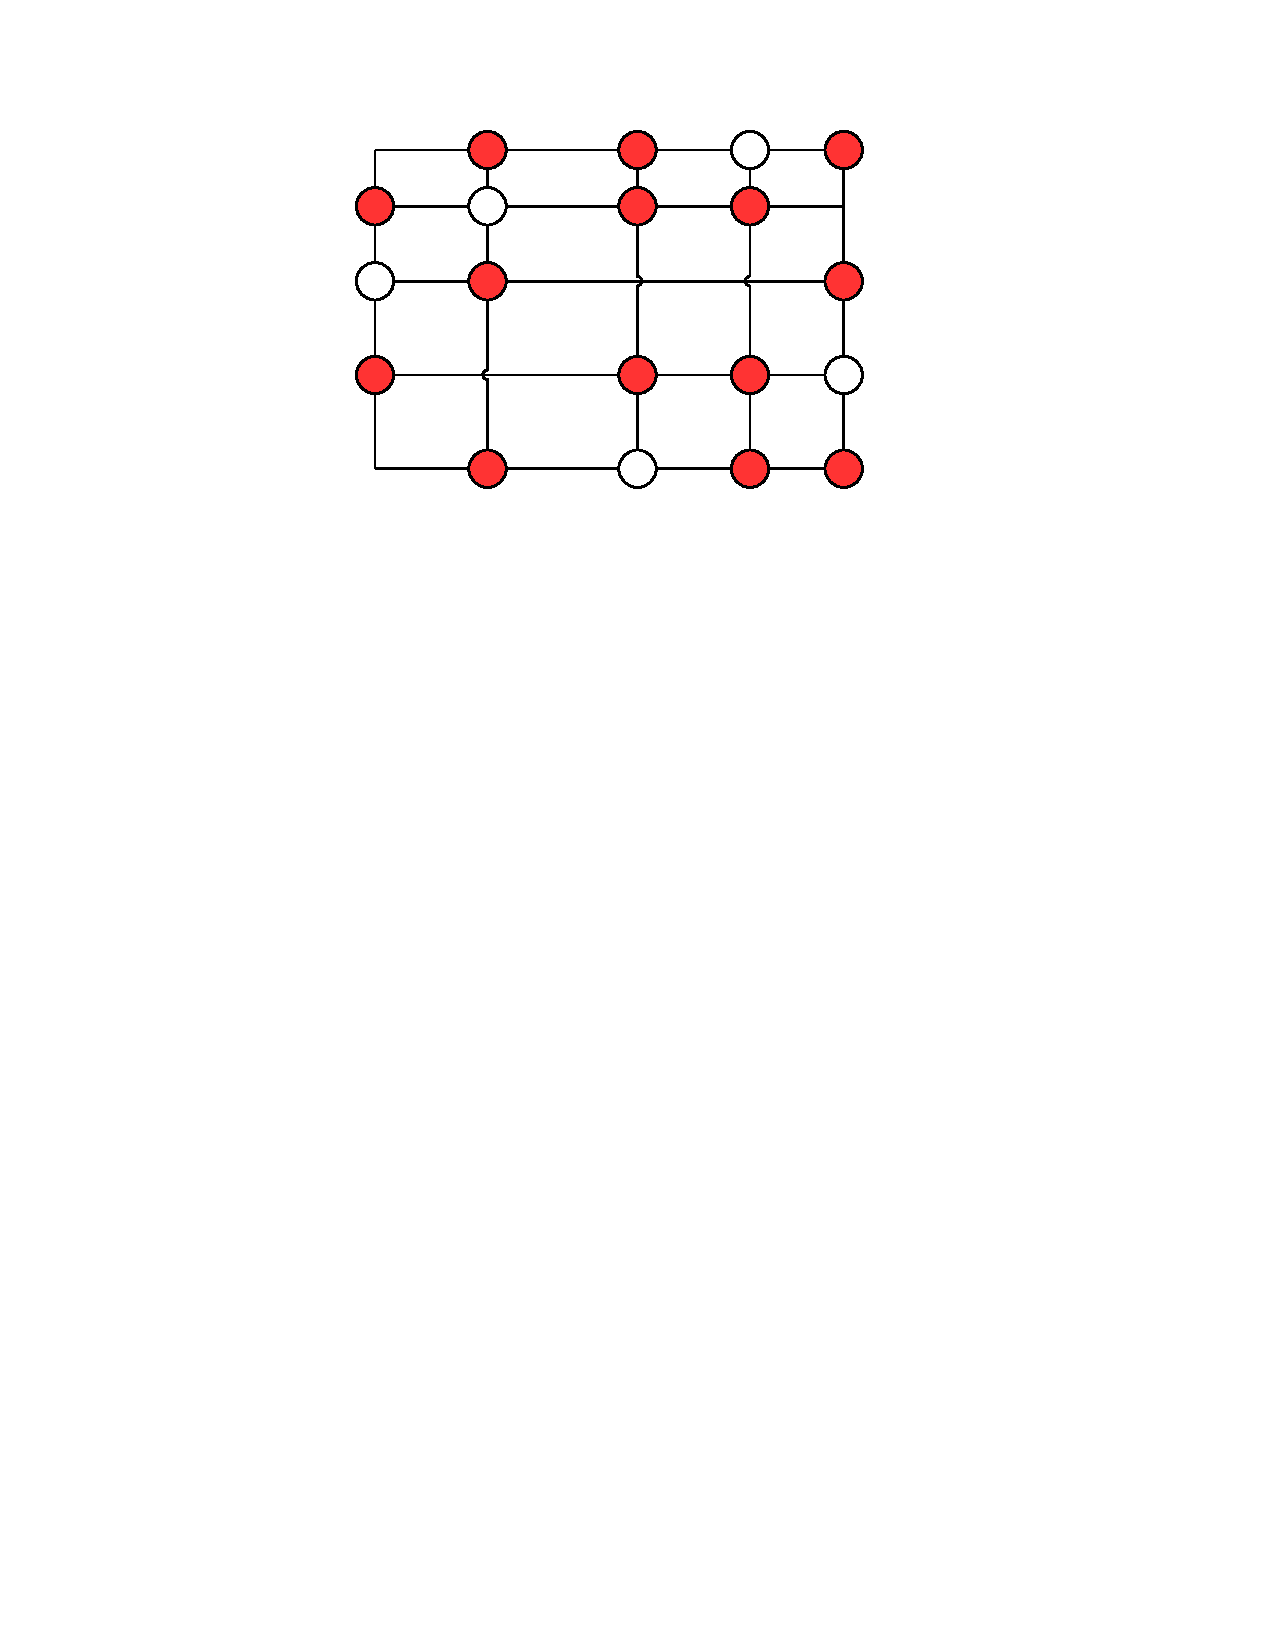
\includegraphics[width=.4\linewidth]{lpsolution.pdf}\label{fig:lpsolution}}
\caption{Integrality gap of the integer program. White circles represent points in $P$.}
\label{fig:integralitygap}
\end{figure}

To illustrate why this is a big problem, suppose we had a rounding scheme from the linear programming relaxation. We call the rounded solution $R$, and we let $LP$ be the optimum of the relaxed linear program, and we let $ILP$ be the optimum of the integer linear program. We know that
\[ LP \leq ILP \leq R \leq O(\log n)LP \]
It would be desirable to show that $R$ is within a constant factor of $ILP$ by bounding it between $LP$ and $O(1)LP$. However, the above formulation will only allow us to show that $R$ is an $O(\log n)$-approximation away from $ILP$.

\section{Extending the Method}

Our hope was to show that this technique of producing an unbounded integrality gap extends to all linear programming interpretations of arboral satisfaction. The intuition we had was that simply changing the weights of the constraint we wrote down or condensing them into fewer constraints should not eliminate an unbounded integrality gap. However, we have been unable to confirm this. In this section, we present a number of observations we have made about general ILP's for the points in the plane problem. 

The assumption we make is that each variable corresponds to one grid point, and vice versa, and that the variable is set to $1$ when the point is included in the set $Q$ and is 0 otherwise. We then know that there must be $n$ constraints that set the $n$ points in $P$ equal to 1, and without loss of generality, we can say that all the other constraints have a RHS of the form $\leq 1$. The last claim is slightly nontrivial, as a scaling / flipping signs argument only guarantees that constraints are of the form $\leq \pm 1$. However, we rule out all constraints of the form $\leq -1$, since this constraint must be satisfied in the case where all variables are set to 0 (since the case of no points on the grid is arborally satisfied, the inequality constraints must be satisfied). 

For the following observations, we use variables to refer to both variables in the linear program, as well as the corresponding points on the grid. This language is not technically correct, but it allows us to state theorems more cleanly.

\begin{observation}
For each pair of points $x$ and $y$ that span a rectangle, there exists a contraint $C$ such that
\[ C: a_1x + a_2y + \dots \leq 1 \]
where $a_1 \leq 1$, $a_2 \leq 1$ and $a_1 + a_2 > 1$. 
\end{observation}

\begin{proof}
This follows from the fact that if there is only one point, the set is arborally satisfied. This means that all positive coefficients are less than or equal to $1$. Also, the point set where $x$ and $y$ are the only two points present is not arborally satisfied, so plugging in $x = y = 1$ and setting all variables equal to 0 must violate this constraint. This gives $a_1 + a_2 > 1$.
\end{proof}

\begin{observation}
For each pair of points $x$ and $y$ which span a rectangle, where $z$ is a different point on the corner of the rectangle spanned by $x$ and $y$, we have
\[ C: a_1x + a_2y + a_zz + \dots \leq 1 \]
where $a_1 + a_2 + a_z \leq 1$ and so $a_z < 0$.
\end{observation}

\begin{proof}
This follows from the fact that constraint $C$ was not satisfied in the case where $x = y = 1$ and all other variables are set to 0, but is satisfied when $x = y = z = 1$, and all other variables are set to 0. We see that $a_1 + a_2 > 1$ and $a_1 + a_2 + a_1 \leq 1$ implies $a_z < 0$. \end{proof}

In fact, we can make a more general version of this statement.

\begin{observation}
For each pair of points $x$ and $y$ which span a rectangle, let $z_1$ and $z_2$ be points on the edge of the rectangle that are directly across from each other. Then we have 
\[ C : a_1x + a_2y + a_{z_1}z_1 + a_{z_2}z_2 + \dots \leq 1\]
where $a_1 + a_2 + a_{z_1} + a_{z_2} \leq 1$ and so $a_{z_1} + a_{z_2} < 0$. 
\end{observation}

\begin{proof}
Identical to the proof of Observation 2, but now with an extra variable. \end{proof}

We wanted to use observations such as these to make more specific statements about the structure of the constraints, which would have allowed us to come up with (possibly weighted) variants of the feasible solution from Section 6.

\begin{comment}
We make three assumptions about ``natural" linear programs for this problem:

1) Grid points should correspond to variables and vice versa, and variables should be 0 or 1 depending on whether or not the grid point is present.

2) There should be one constraint for each possible grid rectangle. It does not seem like it makes sense for a given rectangle's arboral satisfaction to rely on two or more constraints.

3) The structure of the constraint does not depend on the rectangle that corresponds to it. Essentially, this is just assuming that we can write down all constraints in a general form, as we do with equations (1), (2), (3), and (4).

Whether or not these assumptions are sufficiently general or even reasonable is unclear. However, the two linear programs we have shown clearly meet these assumptions, and we believe there is likely an unbounded integrality gap for all programs that do meet these assumptions.

Consider the constraint corresponding to some given positive rectangle defined by two corner vertices $b_{ij}$ and $b_{kl}$ where $i<k$ and $j< l$. We know what points (in constraint space, not the plane) should satisfy the constraints and what do not, so we can use this information to reveal the structure of the constraint. In particular, if at least one of $b_{ij}$ or $b_{kl}$ is 0, the point (in constraint space) should satisfy the constraint no matter what. However, if both $b_{ij}$ and $b_{kl}$ are 1, then we don't want this to be a satisfying arrangement unless some other $b$ within the rectangle is set to 1. Since we can satisfy the rectangle by including any $b$ in the rectangle, we note that the coefficients of these $b$'s must be the opposite of the coefficients on $b_{ij}$ and $b_{kl}$. WLOG, assume the coefficients on $b_{ij}$ and $b_{mn}$ are positive (otherwise we can just multiply both sides by -1), and this tells us the LHS of the constraint is of the form
\[ w_{ij}b_{ij} + w_{kl}b_{kl} - \sum_{b_{mn} \in \text{rectangle}} w_{mn}b_{mn} \]

If no points in the plane are present, the constraints should all be satisfied. We consider the following idea:

For each point $b_{ij}$ in the given point set $P$, increase $b_{i+1,j}$ by $w_{i,j}/w_{i+1,j}$, and increase $b_{i-1,j}$ by $w_{i,j}/w_{i-1,j}$. We can easily check that this leads every LHS of every constraint corresponding to a rectangle formed by two points in $P$ to equal 0. If we could guarantee this for all rectangles, then we would be finished.
\end{comment}

\section{Conclusions}

Our results have shown that the natural linear programming interpretations of the points in the plane do not seem to be particularly helpful in solving the points in the plane problem. Most of the standard methods of tackling linear programs failed, and so we turned our attention to trying to show that perhaps linear programs are not the way to approach this problem. We were able to show an unbounded integrality gap for the specific LP we studied, and we hope that our ideas can be extended to eliminate more general classes of LPs from consideration.

\bibliography{references}
\bibliographystyle{plain}

\end{document}
